% lecture04.tex — Submersions

\section{Submersions}

\begin{definition}{Submersion}{submersion}
    $f \colon M \to N$ is called a \emph{submersion} at $p \in M$ if $df_p$ is surjective. If it is a submersion at every point, it is simply called a \emph{submersion}.
\end{definition}

\begin{theorem}{Local Submersion Theorem}{local-submersion-thm}
    If $f \colon M \to N$ is a submersion at $p \in M$, then there exist local coordinates around $p \in M$ and $f(p) \in N$ such that
    \[
        f(x_1, \ldots, x_m) = (x_1, \ldots, x_n).
    \]
\end{theorem}

\begin{proof}
    Just as in the proof of the local immersion theorem, we start from local parametrizations
    \[
    \begin{tikzcd}
        M \arrow[r, "f"] & N \\
        U \arrow[u, "\phi"] \arrow[r, "g"'] & V \arrow[u, "\psi"']
    \end{tikzcd}
    \]
    where $U \subset \R^m$, $V \subset \R^n$, $\phi(0) = p$, $\psi(0) = f(p)$, and $g = \psi^{-1} \circ f \circ \phi$.

    By the assumption, $dg_0 \colon \R^m \to \R^n$ is surjective, so by change of basis in $\R^m$, we may assume
    \[
        dg_0 = \begin{pmatrix} I_n & 0 \end{pmatrix}
    \]
    where $I_n$ is the $n \times n$ identity and $0$ is $n \times (m - n)$.

    Now define $G \colon U \to \R^m$ by
    \[
        x \mapsto (g(x), x_{n+1}, \ldots, x_m).
    \]
    Then $dG_0 = I_m$, and $G$ is a local diffeomorphism at $0$.

    Note also that $g = \pi \circ G$, where $\pi \colon \R^m \to \R^n$, $(x_1, \ldots, x_m) \mapsto (x_1, \ldots, x_n)$, is the canonical submersion.

    It follows that, after shrinking $U$ and $V$ sufficiently, we have
    \[
    \begin{tikzcd}
        M \arrow[r, "f"] & N \\
        U \arrow[u, "\phi \circ G^{-1}"] \arrow[r, "\pi"'] & V \arrow[u, "\psi"']
    \end{tikzcd}
    \]
    as desired.
\end{proof}

\begin{corollary}{Submersion is an Open Condition}{submersion-open}
    If $f$ is a submersion at $p$, then it is a submersion in a neighborhood of $p$. That is, \emph{submersion is an open condition}.
\end{corollary}

\subsection{Regular and Critical Values}

\begin{definition}{Regular Value}{regular-value}
    For a smooth map $f \colon M \to N$ of manifolds, a point $q \in N$ is called a \emph{regular value} for $f$ if $df_p \colon T_p M \to T_q N$ is surjective at every point $p \in f^{-1}(q)$.
\end{definition}

\begin{theorem}{Preimage Theorem}{preimage-thm}
    If $q$ is a regular value of $f \colon M \to N$, then the preimage $f^{-1}(q)$ is a submanifold of $M$ with dimension
    \[
        \dim f^{-1}(q) = \dim M - \dim N.
    \]
\end{theorem}

\begin{proof}
    For any $p \in f^{-1}(q)$, thanks to the local submersion theorem, we can choose local coordinates around $p$ and $q$ so that
    \[
        f(x_1, \ldots, x_m) = (x_1, \ldots, x_n).
    \]
    Thus, near $p$, $f^{-1}(q)$ is just the set of points $(0, \ldots, 0, x_{n+1}, \ldots, x_m)$, and the functions $x_{n+1}, \ldots, x_m$ form a local coordinate system on a neighborhood of $p \in f^{-1}(q)$.
\end{proof}

\begin{definition}{Critical Value}{critical-value}
    A point $q \in N$ that is not a regular value is called a \emph{critical value}.
\end{definition}

Later, we'll learn that the set of critical values is measure zero (Sard's theorem), so almost every point in $N$ is a regular value of $f$.

\begin{example}{Regular and Critical Values}{reg-crit-examples}
    \begin{enumerate}
        \item $\R^2 \to \R$, $(x,y) \mapsto x^2 + y^2$. The only critical value is $0$.

        \begin{center}
        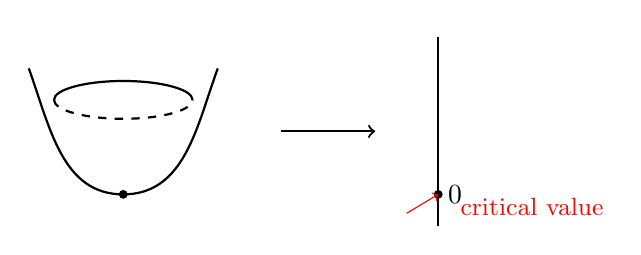
\begin{tikzpicture}[scale=0.8]
            % Paraboloid sketch
            \draw[thick] (-1.5,2.5) to[out=-70,in=180] (0,0.5) to[out=0,in=250] (1.5,2.5);
            \draw[thick,dashed] (-1.1,2) arc(180:360:1.1 and 0.3);
            \draw[thick] (-1.1,2) arc(180:0:1.1 and 0.3);
            \fill (0,0.5) circle (2pt);
            % Arrow
            \draw[->,thick] (2.5,1.5) -- (4,1.5);
            % R line
            \draw[thick] (5,0) -- (5,3);
            \node[right] at (5,3) {$\R$};
            \fill (5,0.5) circle (2pt) node[right] {$0$};
            \node[right,red] at (5.2,0.3) {\small critical value};
            \draw[<-,red] (5,0.5) -- (4.5,0.2);
        \end{tikzpicture}
        \end{center}

        \item $T^2 \to \R$ (height function on the torus). There are critical values at the top, bottom, and the two saddle points.

        \begin{center}
        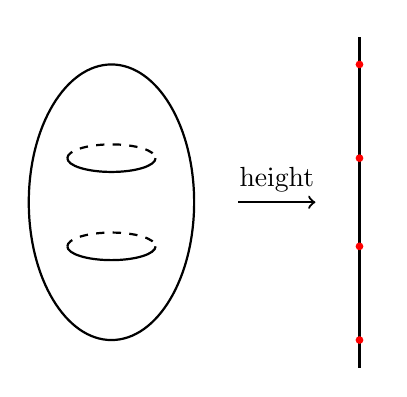
\begin{tikzpicture}[scale=0.7]
            % Torus outline (side view)
            \draw[thick] (0,0) ellipse (1.5 and 2.5);
            \draw[thick] (-0.8,0.8) arc(180:360:0.8 and 0.25);
            \draw[thick,dashed] (-0.8,0.8) arc(180:0:0.8 and 0.25);
            \draw[thick] (-0.8,-0.8) arc(180:360:0.8 and 0.25);
            \draw[thick,dashed] (-0.8,-0.8) arc(180:0:0.8 and 0.25);
            % Arrow
            \draw[->,thick] (2.3,0) -- (3.7,0) node[midway,above] {height};
            % R line
            \draw[thick] (4.5,-3) -- (4.5,3);
            \node[right] at (4.5,3) {$\R$};
            % Critical values
            \foreach \y/\lab in {2.5/top, 0.8/saddle, -0.8/saddle, -2.5/bottom} {
                \fill[red] (4.5,\y) circle (2pt);
            }
        \end{tikzpicture}
        \end{center}
    \end{enumerate}
\end{example}

\subsection{Application: Fundamental Theorem of Algebra}

As an application of these notions, let's prove the \emph{fundamental theorem of algebra}: every non-constant complex polynomial $P(z)$ must have a zero.

First, observe that if $M$ is compact, $q \in N$ is a regular value, and $\dim M = \dim N$, then $f^{-1}(q)$ is a finite set. Moreover, $\# f^{-1}(q)$ is a locally constant function of $q$ (as $q$ ranges only through regular values). (If $p_1, \ldots, p_k$ are points of $f^{-1}(q)$, then we can choose pairwise disjoint neighborhoods $U_1, \ldots, U_k$ mapping diffeomorphically onto $V_1, \ldots, V_k$. We may then take $V = V_1 \cap \cdots \cap V_k - f(M - U_1 - \cdots - U_k)$.)

\begin{proof}[Proof of the fundamental theorem of algebra]
    Consider the unit sphere $S^2 \subset \R^3$ and the stereographic projection
    \[
        h_+ \colon S^2 \setminus \{(0,0,1)\} \to \R^2 \times 0 \subset \R^3.
    \]
    \begin{center}
    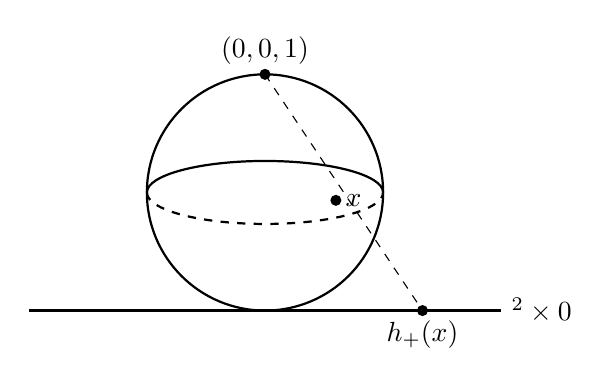
\begin{tikzpicture}[scale=1.0]
        % Sphere
        \draw[thick] (0,0) circle (1.5);
        \draw[thick,dashed] (-1.5,0) arc(180:360:1.5 and 0.4);
        \draw[thick] (-1.5,0) arc(180:0:1.5 and 0.4);
        % North pole
        \fill (0,1.5) circle (2pt) node[above] {$(0,0,1)$};
        % Plane
        \draw[thick] (-3,-1.5) -- (3,-1.5) node[right] {$\R^2 \times 0$};
        % Projection line
        \draw[dashed] (0,1.5) -- (2,-1.5);
        \fill (0.9,-0.1) circle (2pt) node[right] {$x$};
        \fill (2,-1.5) circle (2pt) node[below] {$h_+(x)$};
    \end{tikzpicture}
    \end{center}

    We identify $\R^2 \times 0$ with $\mathbb{C}$. Say $P(z) = a_0 z^n + a_1 z^{n-1} + \cdots + a_n$ with $a_0 \neq 0$.

    The polynomial map $P \colon \mathbb{C} \to \mathbb{C}$ corresponds to the map
    \begin{align*}
        f \colon S^2 &\to S^2 \\
        x &\mapsto h_+^{-1} \circ P \circ h_+(x) \quad \text{for } x \neq (0,0,1), \\
        (0,0,1) &\mapsto (0,0,1).
    \end{align*}

    The resulting map is smooth, even in a neighborhood of $(0,0,1)$. (Let $h_-$ be the stereographic projection from the south pole $(0,0,-1)$. Then $h_+ h_-^{-1}(z) = \frac{z}{|z|^2} = \frac{1}{\bar{z}}$, and $h_- \circ f \circ h_-^{-1}(z) = \frac{z^n}{\bar{a}_0 + \bar{a}_1 z + \cdots + \bar{a}_n z^n}$ is smooth at $0$.)

    Moreover, $f$ has only finitely many critical points, since $P'(z)$ is not identically zero. Hence, the set of regular values of $f$ is connected, and thus $\# f^{-1}(q)$ must be constant on this set. Since $\# f^{-1}(q)$ can't be zero everywhere, it is zero nowhere. Thus $f$ is surjective, and $P$ must have a zero.
\end{proof}
